\section{Andere Darstellungsformen der Eulerschen Zahl}
Eine Sache, die mich an fundamentalen Konstanten wie $e$ interessiert, sind ihre zahlreichen Schreibweisen und wie diese sich verhalten. Zum Einen gibt es das Umschreiben in andere Basen / numerische Systeme, welche ich auf Muster und Struktur untersuchen werde. Zum Anderen existiert die Eulersche Zahl als unendlicher Kettenbruch, welcher abschließend von mir auf seine Näherungsfähigkeit untersucht wird. \subsection{Die Eulersche Zahl in verschiedenen Basen}
Die Eulersche Zahl ist irrational. Für rationale Basen bedeutet dies, dass die Zahl unendlich viele nicht-wiederholende Nachkommastellen aufweist. Diese untersuche ich im folgenden Abschnitt auf Verteilung und Muster und was das für die Zahl bedeutet.
\subsubsection{Basis 10}
In der Basis 10 (in welcher man sich auch normalerweise befindet, ) gibt es 10 Ziffern von 0 bis 9. Untersucht man diese auf Verteilung/Häufigkeit, dann stellt man schnell fest, dass die Eulersche Zahl keine Ziffer bevorzugt und auch keine Muster in der Form von Zifferfolgen aufweist. Dies ist ein erwartetes Verhalten, denn $e$ ist ja irrational.
\begin{figure}[h]
  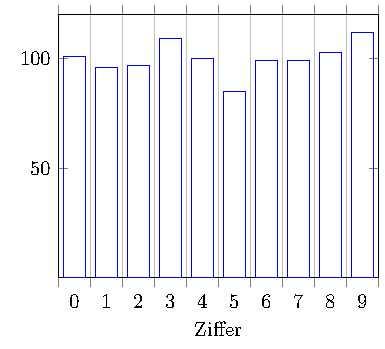
\includegraphics{medien2/basis10/basis10.pdf}
  \centering
\end{figure}
\par In dem Graphen ist die Verteilung von Ziffern der ersten 1000 Stellen von $e$ zu sehen. Zu beachten ist, dass die Y-Achse bei 80 startet (für bessere Erkennbarkeit) und das zum Beispiel die Ziffer 5 mit 85 mal in dem Abschnitt am Wenigsten vorkommt und die Ziffer 9 mit 112 Mal am Meisten.
\subsubsection{Basis 2}
In der Basis 2 ist das gleiche erkennbar. Ziffer 1 und 0 kommen ungefähr gleich oft vor. \subsection{Die Eulersche Zahl als unendlicher Bruch}

